\chapter{Introducci\'on}
\label{chap:intro}
\minitoc

En las ciencias de la computación los lenguajes juegan un rol muy importante en muchas disciplinas. Desde los comienzos se buscaron mecanismos para describirlos y manejarlos, esta rama de la informática ha logrado muchos avances en el tema.

Dentro de los mecanismos desarrollados, las gramáticas han logrado ocupar unos de los lugares más destacados. La continua evolución y descubrimientos de nuevas gramáticas necesitó que se organizaran, y no fue hasta 1956 que Noam Chomsky propuso una jerarquía sobre las gramáticas.

Las clasificó en 4 niveles:

\begin{figure}[h!]\centering 
\begin{tabular}{| c | p{3.5cm} | p{3.5cm} | p{2.4cm} | p{2.9cm}|}
\hline

\rowcolor{gris} \textbf{Tipo} & \textbf{Lenguaje} & \textbf{Autómata} & \textbf{Gramática} &  \textbf{Restricciones} \\ \hline

\multirow{2}{*}{\textbf{0}} & Recursivamente   & Máquina de  & \multirow{2}{*}{Irrestrictas} & \multirow{2}{*}{Sin restricciones} \\ 
                            & enumerable (LRE) & Turing (MT) & &  \\ \hline

\multirow{2}{*}{\textbf{1}} & Dependiente del & Autómata lineal- & Dependiente &\multirow{2}{*}{$\alpha A \beta \rightarrow \alpha\gamma\beta$} \\ 
                            & contexto (LSC)  & mente acotado              & de  contexto & \\ \hline

\multirow{2}{*}{\textbf{2}} & Independiente del & \multirow{2}{*}{Autómata con pila} & Independiente & \multirow{2}{*}{$A \rightarrow \gamma$} \\ 
                            & contexto (LLC)    &           & de contexto& \\ \hline

\multirow{2}{*}{\textbf{3}} & \multirow{2}{*}{Regular (RL)} & \multirow{2}{*}{Autómata finito} & \multirow{2}{*}{Regular} &$A \rightarrow aB$ \\ 
                            &              &                 & & $A \rightarrow a$ \\ \hline
\end{tabular}\caption{\label{chomsky} Jerarquía de Chomsky}
\end{figure}

Desde que D. Knuth introdujo en 1966 las gramáticas de atributos (GA), estas se han utilizado ampliamente para el desarrollo de herramientas de procesamiento de lenguajes formales como compiladores, intérpretes, traductores como también para especificar la semántica de lenguajes de programación.

En el desarrollo de este capítulo, introductorio, abordaremos un amplio numero de conceptos desde un punto de vista informal. A partir del capítulo 2 hasta el 4 inclusive se analizaran algunos de ellos, con mas formalidad y los siguientes capítulos estarán destinados al desarrollo de \maggen. 

\maggen\ es el objetivo principal del proyecto y su denominación esta dada por la combinación de las silabas \textbf{mag}, que significa \textit{multi-plans attribute grammar} y \textbf{Gen} por \textit{generator}. Estas dos silabas dan significado a \maggen\ como ``Generador de Evaluadores Estáticos para MAG''.

\section{Gramática libre de contexto}
En el nivel 2 de la jerarquía de chomsky (fig. \ref{chomsky}) se encuentran los lenguajes libres de contexto. Las gramáticas libres de contexto (CFG) son un formalismo que permite expresar cadenas de este tipo de lenguajes.

Las gramáticas libres de contexto han tomado gran importancia en la descripción de formatos de documentos\footnote{DTD - document-type definition.}, como XML (eXtensible Markup Language) y también en tecnología de compilación, mediante la construcción de \textit{parser} de lenguajes (Ver \cite{compiladores}).  
\begin{definition}
Una gramática libre de contexto se conforma de 4 componentes necesarios para la descripción de un lenguaje:
\begin{enumerate}
\item Un conjunto finito de símbolos que son los string que se definen el lenguaje. Este conjunto es denominado ``alfabeto de terminales'' o simplemente \textit{\textbf{símbolos terminales}}.

\item Un conjunto finito de variables llamados \textit{\textbf{símbolos no terminales}} o ``categorías sintácticas''. Cada uno de estos define un lenguaje, es decir un conjunto de strings.

\item Una variable que representa el comienzo del lenguaje, que se denomina \textit{\textbf{símbolo inicial}}. Dicha variable pertenece al conjunto del punto 2.

\item Un conjunto finito de \textit{\textbf{producciones o reglas}} que representan la definición recursiva de un lenguaje. Cada producción consiste de las siguientes partes:

\begin{enumerate}
\item Un símbolo no terminal perteneciente al conjunto del punto 2, denominado \textit{\textbf{head}} de la producción.

\item El símbolo \textbf{$\rightarrow$}.

\item Una secuencia de 0 o mas símbolos no terminales y terminales. Este, es denominado \textit{\textbf{body}} de la producción y representa el string formado por el \textit{head}.
\end{enumerate}

\end{enumerate}

Estos cuatro componentes pueden ser representados por una tupla \textbf{<V,T,S,P>}\ donde \textbf{V} es el conjunto de no terminales (punto 1), \textbf{T} el conjunto de terminales (punto 2), \textbf{S} es el símbolo inicial (punto 3) y \textbf{P} es el conjunto de producciones (punto 4).
\end{definition}
\underline{Nota:}
En todo el desarrollo del trabajo se denotara a los símbolos no terminales con letras en mayúscula y a los símbolos terminales con letras en minúscula para mayor claridad.
Veamos dos ejemplos desarrollados en \cite{gramática} (capítulo 5):

\begin{enumerate}
\item Ejemplo: palíndromo:
Definimos la gramática $G_{pal}$ para definir el lenguaje de palíndromos\footnote{Un palíndromo (del griego \textit{palin dromein}, volver a ir hacia atrás) es una palabra, número o frase que se lee igual hacia adelante que hacia atrás. Si se trata de un número, se llama capicúa (\urllink{http://es.wikipedia.org/wiki/Palíndromo}).}: \\
$G_{pal} = (\{P\},\{0,1\},P,A)$
donde A es el siguiente conjunto de producciones:
\begin{enumerate}
\item $P \rightarrow \lambda$
\item $P \rightarrow 0$
\item $P \rightarrow 1$
\item $P \rightarrow 0 P 0$
\item $P \rightarrow 1 P 1$
\end{enumerate}
Ejemplos de cadenas del lenguaje $G_{pal}$:
\begin{items}
\item $\lambda$
\item 0011
\item 11110000
\item etc.
\end{items}

\item Ejemplo: Gramática de expresiones:\\
\textbf{G = (\{E,I\}, \{+,*,(,),a,b,0,1\}, E, P)} donde P es el conjunto de producciones siguiente:
\begin{enumerate}
\item $E \rightarrow I$
\item $E \rightarrow E + E$
\item $E \rightarrow E * E$
\item $E \rightarrow (E)$
\item $I \rightarrow a$
\item $I \rightarrow b$
\item $I \rightarrow Ia$
\item $I \rightarrow Ib$
\item $I \rightarrow I0$
\item $I \rightarrow I1$
\end{enumerate}
\begin{items}
\item a
\item b00
\item a*(a+b00)
\item etc.
\end{items}
\end{enumerate}

\underline{Abreviación de reglas}: Cuando denotamos una producción podemos utilizar una abreviación para agrupar aquellas producciones con el mismo \textit{head}. Para ello utilizamos el metasímbolo ``|''. Por ejemplo el conjunto de producciones de $G_{pal}$ podríamos escribirlas como: $P \rightarrow \lambda | 0 | 1 | 0P0 | 1P1$ 

\underline{Observación:}
De aquí en adelante se asumirá que el símbolo de comienzo $ S $  aparece en la parte izquierda de una única producción y no puede aparecer en la parte derecha de ninguna producción\footnote{Esta forma se denomina \emph{forma normal} o también \textit{Gramática extendida}.}. \\

\begin{definition} Se dice que una gramática libre de contexto $G=<V,T,S,P>$
es \textbf{reducida} si
$\forall B \in V$ , $\exists \alpha , \gamma \in \Sigma^{*} : S \clausderiva{G} \alpha B \gamma$ y $\exists \tau \in T^{*} : B \clausderiva{G} \tau$.
\label{def:reducida}
\end{definition}

\begin{definition} 
Dada una gramática $G = <V,T,P,S>$ definimos $ST = (K,D)$ como un árbol de derivación (o parse tree) donde $K$ es un conjunto de nodos y $D$ es una relación no reflexiva sobre $K$), con $k_0$ como raíz; si cumple las siguientes condiciones:
\begin{items}
\item $ K \subseteq (V \cup T \cup \epsilon) $
\item $k_{0}$ es un rótulo raíz para el símbolo S.
\item $ S \rightarrow k_{1} \ldots k_{n} $ donde $k_{1} \ldots k_{n}$ son rótulos para los símbolos de la parte derecha de la producción.
\item Si $k_{i} \in T \cup \{\epsilon\}$, ($1 \leq i \leq n$), entonces $k_{i}$ es una hoja de $ST$.
\item Si $k_{i} \in V$,  ($1 \leq i \leq n$), entonces $k_{i}$ es la raíz del 
      árbol sintáctico para la gramática libre de contexto $<V,T,P,K_I>$, donde $K_{I}$ es un rótulo para $k_{i}$.
\end{items}
\label{def:arbolderivacion}
\end{definition}

\begin{definition} Una gramática libre de contexto $G = <V,T,S,P>$ es \textbf{ambigua} si para una cadena $\alpha$, derivada de $G$, existen dos o más árboles de derivación diferentes.
\label{def:ambigua}
\end{definition}

\section*{Notación}

La notación usada tanto en el desarrollo del proyecto, comunicación entre los autores y redacción de este informe es la utilizada por Wuu yang en \cite{wuu-yang1}, la cual proviene de la notación de Kastens en \cite{kastens} y la utilizada por el Mg. Marcelo Arroyo en \cite{tesismarcelo}

\section{Gramática bien formada}

Una gramática bien formada\footnote{En inglés Well Defined, de allí la abreviatura WD.}, es una gramática que no contiene directa o indirectamente reglas recursivas a izquierda.

Esta propiedad estructural verificable implica la completitud, siempre y cuando se sea lo suficientemente permisivo para muchos propósitos.

Una gramática puede tener reglas recursivas a izquierda, pero seguirá siendo completa si su ciclo se degenera y se vuelve inalcanzable.

\begin{definition}
Definimos inductivamente al conjunto $WF_{G}$ (\textbf{well formed grammar}) como sigue. Escribimos WF(\textbf{e}) a $ \textbf{e}\in WF_{G}$ que significa la expresión \textbf{e} es \textbf{well formed} o bien formada en G.
\begin{enumerate}
\item $ WF(\varepsilon)$
\item $ WF(a)$
\item $ WF(A)$ si $WF ( R_{G}(A))$
\item $ WF(e_{1}e_{2})$ si $ WF(e_{1})$ y $e_{1}\rightarrow 0$ implica $ WF(e_{2})$
\item $ WF(e_{1}/e_{2})$ si $ WF(e_{1})$ y $ WF(e_{2})$
\item $ WF(e^{*})$ si $ WF(e)$ y $ e\not\rightarrow 0$
\item $ WF(!e)$ si $ WF(e)$
\end{enumerate}
\end{definition}

\section{Gramática de Atributos}

Las Gramáticas de Atributos (GA) son un formalismo simple para la especificación de la semántica de lenguajes formales, como los lenguajes de programación o de especificación. Integran la modularidad que brindan las gramáticas libres de contexto y la expresividad de un lenguaje funcional.

En una gramática de atributos, se relaciona con cada símbolo de una gramática libre de contexto un conjunto de atributos. Cada regla o producción tiene asociados un conjunto de reglas semánticas que toman la forma de asignación a atributos de valores denotados por la aplicación de una función, la cual puede tomar como argumentos instancias de atributos pertenecientes a los símbolos que aparecen en la producción.
Las reglas semánticas inducen dependencias entre los atributos que ocurren en la producción. El orden de evaluación es implícito (si existe) y queda determinado por las dependencias entre las instancias de los atributos.
Una regla semántica se podrá evaluar cuando las instancias de los atributos que aparecen como sus argumentos estén evaluadas. La noción de orden de evaluación es detallada en la sección \ref{sec:met_eval}

\begin{definition}
\label{def:grammarattr}
Una gramática de atributos es una tupla GA = (G, A, V, Dom, F, R) donde:
\begin{itemize}
\item G = (VN , VT , S, P ) es una CFG reducida y no ambigua (Ver definiciones \ref{def:arbolderivacion} y \ref{def:reducida}).
\item A = $\cup_{X\in(VN \cup T)} A(X)$, es el conjunto finito de atributos (A(X) es el conjunto de atributos asociados al símbolo X)

\item V es el conjunto finito de dominios de valores de los atributos.
\item Dom : $A\rightarrow V$ asocia a cada atributo un dominio o conjunto de valores d $\in$ V .
\item F es un conjunto finito de funciones semánticas de la forma:
\begin{equation}
f \subseteq (\bigotimes\limits_{j=0}^{k}{ Dom(a_{j} ))\rightarrow Dom(a_{0})}
\end{equation}

\item R = $\bigcup _{p \in P} R^{p}$ es el conjunto finito de reglas de atribución o ecuaciones asociadas a cada producción p $\in$ P , donde
\begin{equation}
R^{p} = \bigcup\limits_{j=0}^{m^{p}}{\{r_{j}^{p}\}}\ \ \ \ \ \ (\#(R^{p} ) = m^{p} \geq 0)
\end{equation}
y cada regla $r_{j}^{p} \in R^{p}$ , con 0 $\leq$ j $\leq$ $m^{p}$ es de la forma

\begin{equation}
r_{j}^{p}: X_{0}.a_{0} = f(X_{1}.a_{1} ,\dots , X_{k}.a_{k})
\end{equation} 
donde cada $X_{i}$ es un símbolo que ocurre en la producción \textit{p} , $a_{i} \in A(X_{i})$, ($0 \leqslant i \leqslant k$) y $f \in F$.

\end{itemize}
\end{definition}

\begin{definition} Un atributo $a$ está asociado al símbolo $X$ si y sólo si $a \in A(X)$. 
\end{definition}
\underline{Nota:}
Se utilizará la notación \textbf{X.a} para significar que el atributo \texttt{a} está asociado al símbolo \texttt{X} (a $\in$ A(X)) y para denotar el valor de una ocurrencia o instancia del atributo \texttt{a} del símbolo \texttt{X} en una regla de atribución

\section{Árbol sintáctico}

Un árbol sintáctico abstracto (AST) es una forma condensada de un árbol de análisis sintáctico. Estos son sumamente útiles para representar construcciones del lenguajes.

Por ejemplo una producción de la forma:
\begin{center}\large
$S\ \rightarrow\ \textbf{if}\ B\ \textbf{then}\ S1\ \textbf{else}\ S2$                                                                      \end{center}
puede aparecer en un árbol sintáctico como:

\begin{figure}[h!]\centering
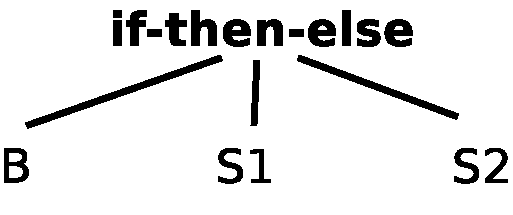
\includegraphics[width=125pt,height=53pt]{ast-ejemplo.pdf}
\caption{\label{ejem-ast} Ejemplo AST.}
\end{figure}
\begin{definition}

Dado una gramática G= \textbf{<V,T,S,P>}\, un árbol de derivación (o árbol sintáctico)
ST(G) es un árbol que se compone de dos tipos de nodos:
\begin{description}

\item [Nodos hojas] Cada nodo hoja es nombrada por una variable en T o por $\lambda$. En caso de que el nodo se nombre con $\lambda$, este es el único hijo del nodo padre.

\item [Nodos interiores] Cada nodo interior es nombrado por una variable en V. Dado $A\in V$ y $p\in P$ de la forma $A\rightarrow X_{1},X_{2},\dots, X_{k}$ el node \textbf{A} tendrá los hijos $X_{1},X_{2},\dots, X_{k}$
\end{description}
\end{definition}

\subsection*{Árbol Sintáctico atribuido}

Un árbol sintáctico atribuido es un AST que agrega información a los nodos, para almacenar los atributos de cada símbolo.
Para una mayor claridad, definimos un nodo del árbol como una tupla $(X_{0}.a_{0}, (X_{1}.a_{1}, X_{2}.a_{2}, \ldots , X_{k}.a_{k}))$ donde $(X_{0}.a_{0})$ es el rótulo y $(X_{1}.a_{1}, X_{2}.a_{2}, \ldots , X_{k}.a_{k})$ son los nodos hijos.

Diremos que en un nodo $n = (X_{0}._{a0}, (X_{1}.a_{1}, X_{2}.a_{2}, \ldots, X_{k}.a_{k}))$ cada $X_{i}.a_{i}$, $(1 \leq i \leq k)$, es una instancia del atributo $X_{i}.a_{i}$, en la gramática.

\begin{definition} 
\label{def:ast-attr}
El árbol atribuido, sobre el cual las instancias de los atributos en cada nodo han sido definidas (es decir, cada instancia se ha asociado a un valor de su dominio), se
denomina \textbf{árbol decorado}.
\end{definition}

\begin{definition} Para un árbol sintáctico atribuido $T(GA)$, su grafo de dependencias $GD(T)$ es el grafo construido a partir de la composición de los grafos de dependencias $GD(p)$ de cada producción aplicada durante la construcción de $T$. Formalmente,

$GD(T)=(V_{GD}(T),E_{GD}(T))$

donde:

\begin{enumerate}
\item $ V_{GD}(T) = \{ X.a \mid \exists n, $ un nodo de T(GA) con 
      rótulo $ X $ y $a \in A(X)$..
      
\item La relación $ E_{GD}(T) $ (arcos de $ GD(T) $) cumple con la siguiente 
      propiedad:

      Sea $n$ un nodo de $T(GA)$ con rótulo $X_0$, cuyos hijos son los nodos
      $ n_1, n_2, \ldots ,n_k $, con $ k \geq 0 $ con rótulos 
      $ X_1 $, $ X_2 $, $\ldots$, $ X_k $, respectivamente, y sea 
      $p:X_0 \rightarrow X_1 X_2 \ldots X_k$ una producción de GA, entonces,
      
      $ (X_{i}.a,X_{j}.b) \in E_{GD}(T) \Leftrightarrow 
         (X_{i}.a,X_{j}.b) \in DP(p) \hspace{0.5cm} 0 \leq i, \: j \leq k $
donde DP(p) se define como:

$DP(p) = \{(X_{i}.a,X_{j}.b) \mid X_{j}.b \rightarrow X_{i}.a \in R^{p}\}$

\end{enumerate}
\end{definition}

\section{Métodos de Evaluación}
\label{sec:met_eval}
Un evaluador de gramáticas de atributos debe tener en cuenta las dependencias entre las instancias de atributos para seguir un orden consistente de evaluación de los mismos.
\begin{definition} Un orden de evaluación consistente, con respecto a las dependencias entre los atributos de una gramática de atributos $GA$, es una secuencia (orden parcial) de instancias de atributos con la siguiente restricción:
Dada una regla $r_{j}^{p} : X_{0}.a_{0} = f(\ldots, X_{i}.a_{i}, \ldots)$ en una producción $p$, 
$X_{i}.a_{i}$ deberá preceder a $X_{0}.a_{0}$.
\end{definition}

\begin{definition} Una gramática de atributos $GA$ es circular si y solo si existe un árbol sintáctico atribuido $T(GA)$, tal que su grafo de dependencias $GD(T)$ contiene al menos un ciclo.
\end{definition}

Si una GA contiene dependencias circulares no podría ser evaluada ya que no se encontraría un orden de evaluación. Esto se conoce como el problema de la circularidad, el cual se ha demostrado ser intrínsecamente exponencial\ref{XXX}. El problema de la circularidad ha motivado que muchos investigadores hayan realizado esfuerzos en la búsqueda e identificación de familias o subgrupos de gramáticas de atributos, para las cuales puedan detectarse circularidades con algoritmos de menor complejidad (polinomial o lineal).

Estas familias imponen restricciones sobre la gramática de atributos o sobre las dependencias entre sus atributos para garantizar que una GA no sea circular, con el costo de restringir su poder expresivo.

En 1980, Uwe Kastens\ref{XXX} caracterizó las gramáticas de atributos ordenadas y propuso un método para su evaluación, denominado secuencias de visita. Estas son, secuencias de operaciones que conducen el recorrido del árbol sintáctico atribuido y realizan la evaluación de las instancias de los atributos. Kastens propone un método para generar las secuencias de visita en tiempo polinomial para la familia OAG. Esta familia y otras como las absolutamente no circulares (ANCAG)\ref{XXX} son tratadas en el capítulo 2.

Luego, en 1998, Wuu-Yang en \cite{wuu-yang1} caracteriza una nueva familia denominada \textbf{Gramática de Atributos Multi-plans}, presentado una algoritmo de evaluación basado en secuencia de visita en tiempo polinomial en el numero de símbolos y producciones. Estas, son desarrolladas en el capítulo 3 y son en las que se basa el funcionamientos de \maggen.  

\subsection{Evaluación dinámica}

Un evaluador dinámico tiene como ventajas su simplicidad y que es posible evaluar cualquier WDAG (GA bien definida)\footnote{Esta familia es detalla en el capitulo siguiente (sección \ref{XXX}).} o aún GA’s irrestrictas utilizando \textit{evaluación lazy}\footnote{\urllink{http://en.wikipedia.org/wiki/Lazy\_evaluation}} (siempre y cuando exista el mínimo punto fijo en el álgebra de términos denotado por las ecuaciones de atribución). Además se pueden detectar ciclos en el grafo de dependencias antes o durante la evaluación.

Las principales desventajas son que generalmente es necesario mantener el árbol sintáctico y el grafo de dependencias. La construcción del grafo de dependencias consume tiempo y memoria; y a su vez, el tiempo de procesamiento insumido en la construcción del grafo de dependencias puede ser mayor que el proceso de evaluación en sí mismo. En la practica, si tomamos una GA de un tamaño normalmente usado, los requerimientos de memoria pueden ser considerables.  

La realidad es que, los evaluadores dinámicos no han tenido mucho interés en el desarrollo de herramientas de generación de procesadores de lenguajes (como por ejemplo los compiladores)debido a que uno de los principales requisitos de un compilador es que sea eficiente, ya que durante un desarrollo un programador generalmente necesita recompilar un número muy importante de veces hasta obtener una versión final del programa requerido.

Razón por la cual \maggen\ genera un evaluador estático y debido a esto no profundizaremos demasiado en este tipo de evaluadores.

\subsection{Evaluación estática}
Los métodos estáticos deben tener en cuenta todos los posibles árboles sintácticos posibles a ser generados por la gramática y calcular todas las posibles dependencias entre las instancias de los atributos. 

Un árbol sintáctico se construye a partir de la aplicación sucesiva de producciones de la
gramática. Una instancia de una producción en un árbol sintáctico tiene como
\emph{contexto inferior} a las instancias de las producciones aplicadas a los no terminales de la parte derecha.
Dada una producción $p$ se deben tomar en cuenta tres tipos de dependencias:
\begin{enumerate}
\item Directas obtenidas por las ecuaciones de $p$
\item Impuestas por el contexto superior
\item Impuestas en el contexto inferior
\end{enumerate}

Instancias diferentes de una producción $p$ tendrán las mismas dependencias
directas, pero podrán tener diferentes dependencias impuestas por los contextos
inferiores y superiores. Es necesario entonces, determinar todas las
\emph{dependencias posibles} entre las instancias de los atributos que ocurren
en una producción para luego poder determinar todas los \emph{planes de evaluacion
posibles} entre los atributos que ocurren en una producción.

Entonces, cada plan de evaluacion que computa las dependencias impuestas en una produccion va acompañado con el \textit{contexto} en el cual el mismo se efectua.

Además, se deberán detectar las posibles dependencias circulares, para informar la viabilidad de su evaluación.

\section{Secuencia de visita}
\section{Generación de evaluadores para GA bien definidas}

bla bla

